\documentclass[./thesis.tex]{subfiles}

 
\begin{document}

The diagonalization of the Hamiltonian is a necessary step in configuration
interaction. Standard diagonalization algorithms scale as $\order{\Ndet^3}$ in
terms of computation, and $\order{\Ndet^2}$ in terms of storage, so the cost is
prohibitive as $\Ndet$ ranges usually between a few million and a few billion.

Fortunately,  not all the spectrum of $\hat H$ is required: only the few lowest
eigenstates are of interest. The Davidson algorithm\cite{Davidson_1975} is an
iterative algorithm which aims at extracting the first few $\Nstate$ lowest
eigenstates of a large matrix. This algorithm reduces the cost of the 
computation and the storage to $\order{\Nstate \Ndet^2}$, and is presented as
algorithm~\ref{alg:davidson}.


%TODO mettre ici le pseudocode 


\alert{
\begin{itemize}
\item Raconter ce qu'il y a dans le papier original : [ E.R.  Davidson, J.  Comput.  Phys.  17 (1975) 87 ].
\item Mettre le pseudocode de l'algorithme.
\item Parler de quelques ameliorations depuis : [ J.  Olsen, P.  Joregensen and J.  Simons, Chem.  Phys.  Letters 169 (1990) 463 ], [F.X.  Gadea /Chemical Physics Letters 227 (1994) 201-210] 
\item Dire qu'on utilise l'algorithme original parce qu'on a toujours un bon guess (CIPSI)
\item Pour etre fonction propre de $S^2$ on utilise une penalty method, comme dans [10.1021/acs.jctc.7b00466]. (D'ailleurs dans ce papier il y a un pseudocode pour Davidson). Et tu peux ajouter qu'on calcule $S^2c$ en meme temps que $Hc$.
\end{itemize}
}

    
Algorithmically, the expensive part of the Davidson diagonalization is the computation of the matrix-vector products $\mH \mc$.

Determinants are connected by $\mH$ only if they differ by no more than two
spinorbitals. Therefore, the number of non-zero elements per line of $\mH$ is
equal to the number of single and double excitation operators, namely
$\order{\Nelec^2 \times (\Norb - \Nelec)^2}$. As $\mH$ is symmetric, the number
of non-zero elements per column is identical. This makes the $\mH$ matrix very
sparse, but for large basis sets the whole $\mH$ matrix may not fit in the
memory of a single node, as the number of non-zero entries to store is
$\order{\Ndet \times \Nelec^2 \times (\Norb - \Nelec)^2}$.  One possibility
would be to distribute the storage of Hamiltonian among multiple compute nodes,
and use a distributed library such as PBLAS\cite{pblas} to perform the
matrix-vector operations. Another approach is to use a so-called \emph{direct}
algorithm, where the matrix elements are computed \emph{on the fly}, and this
is the approach chosen in the \QP.


This effectively means iterating over all pairs of determinants $\ki$ and
$\kj$, checking whether $\ki$ and $\kj$ are connected by $\mH$ and if they are,
accessing the corresponding integral(s) and computing the phase factor.  Even
though we presented a very effective method to compute the excitation degree
between two determinants, the number of such computations to be made scales as
$\Ndet^2$, which can still be prohibitively high. To get an efficient
implementation it is mandatory to filter out all pairs of determinants that are
not connected by $\mH$, and iterate only over connected pairs.  We have
implemented an algorithm similar to the \emph{Direct Selected Configuration
Interaction Using Strings} (DISCIUS) algorithm,\cite{Povill_1995} as presented
in algorithm~\ref{alg:hu}.




%%%%%
The base approach to this problem is to sort, or rather classify, determinants so as to build sets that are by construction disconnected from others. Generally speaking, the set of all determinants is split in disjoint sets $S_c$, $c$ being a mathematical object of the set $\mathcal{T}$. $\mathcal{D}$ is the set of determinants. For a specific method, we have the functions
\begin{itemize}
	\item
	$C : \mathcal{D} \rightarrow \mathcal{T}$, a function that takes a determinant and returns a value in $\mathcal{T}$
	\item
	$p : \mathcal{T}^2 \rightarrow \{ \TRUE, \FALSE \}$, a function that takes a pair $(x,y) \in \mathcal{T}^2$, and returns $\FALSE$ if all the determinants of $S_x$ are disconnected to all the determinants of $S_y$, $\TRUE$ otherwise.
	\item
	$D \in S_{C(D)}$
\end{itemize}  

%TODO : J'en suis la 

Although it's not formally needed, it is pretty much necessary in practice to have some comparison operator for elements of $\mathcal{T}$, so that sets can be easily formed by sorting determinants according to their respective $C(D)$. However, the choice for this operator is entirely arbitrary and doesn't affect the method, so it will not be discussed.
    
    
We can then represent the cost of computing $\mH$ using a matrix $\mathbf{M}$ of same size, where each element $M_{ij}=1$ if the corresponding element $H_{ij}$ needs to be computed, and $M_{ij}=0$ if it is known to be zero by construction.

\alert{
Theoretical representation of $\mathbf{M}$ with 3 classes of determinants $A$, $B$, and $C$, $A$ and $C$ being by construction disconnected. $H_{ij}$ elements corresponding to the white area are, by construction, known to be null. Those in the yellow area need to be computed.
}
    
\begin{figure}[h!]
	\begin{center}
		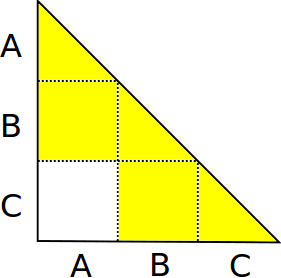
\includegraphics[width=0.4\columnwidth]{figures/davidson/disconnected_classes}
		\caption{{\label{generators_selectors}
		}}
	\end{center}
\end{figure}

Because the number of determinants used in the following examples is 500k, $M$ is shown as a density map.

As an example, one of the first attempted classification was according to the number of electrons in $s$ a subset of orbitals. Indeed, if $\ket I$ has $n$ electrons in an arbitrary subset of orbitals, and $\ket J$ has $n-3$, quite obviously it will take at least 3 excitations to excite from $\ket I$ to $\ket J$.
\begin{itemize}
	\item
	$\mathcal{T}$ is type scalar
	\item
	$C(D)$ returns the number of electrons in the chosen subset.
	\item
	$p(x, y) = |x-y| \leq 2$
\end{itemize}

Computation of $C(D)$ can be acheived using bitstrings. With $S$ a bitstring containing the orbitals wanted in the subset. The number of electrons in this subset for a determinant $\ket I$ represented by a $\alpha \beta$-bitstring $I$ is
\begin{equation}
C(I)=|I_{\alpha} \wedge S|+|I_{\beta} \wedge S|
\end{equation}

Using a subset is equivalent to using the complementary subset, so it is best to pick $N_{orb}/2$ orbitals. For a better entropy, it is of course better to interleave the chosen orbitals.
\begin{equation}
S=binary(...101010101...)
\end{equation}
    
Determinants are sorted according to this criterion. Using ClBr with 500k determinants, and sorting determinant in increasing order of their respecive $C(D)$, we got matrix $M$ shown in figure \ref{fig:num_subspace}

\begin{figure}[h!]
	\begin{center}
		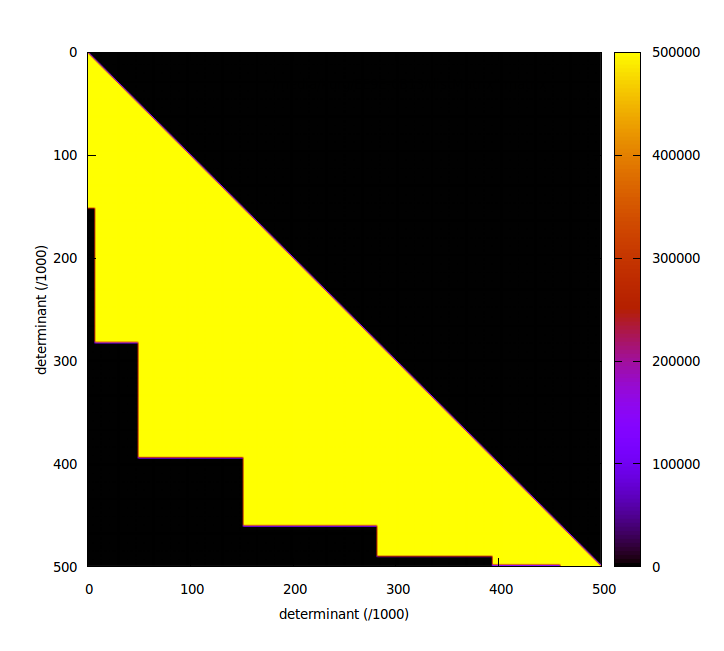
\includegraphics[width=0.6\columnwidth]{figures/davidson/num_subspace}
		\caption{{\label{fig:num_subspace}
		}}
	\end{center}
\end{figure}
    
As expected, the farther away two determinants $\ket I$ and $\ket J$ are in the sorted determinant vector, the likelier it is that $|C(I)-C(J)| > 2$ which makes them disconnected by construction. The "staircase" aspect shows the boundaries of each class.
However, only a relatively small area of $H$ is null by construction. It is possible to further reduce the area to be explored by chosing several orbital subsets $S_1$ to $S_n$ instead of a single one. In this case, $C(D)$ returns $c$ a vector of size $n$ with $c_{i}$ the number of electron in subset $S_i$ for $D$

\begin{itemize}
	\item
	$\mathcal{T}$ is type vector size $n$
	\item
	$C(D)$ returns $c$ a vector of size $n$, $c_i$ the number of electron in subset $S_i$
	\item
	$p(x, y) = |x_i - y_i| \leq 2 \forall i$
\end{itemize}



Using $n=3$ uncorrelated subsets
\begin{equation}
S_1 = binary(...010101010101...)
\end{equation}
\begin{equation}
S_2 = binary(...110011001100...)
\end{equation}
\begin{equation}
S_3 = binary(...111100001111...)
\end{equation}
The resulting $M$ in figure \ref{fig:num_subspace3} looks awesome but the area isn't reduced much.

\begin{figure}[h!]
	\begin{center}
		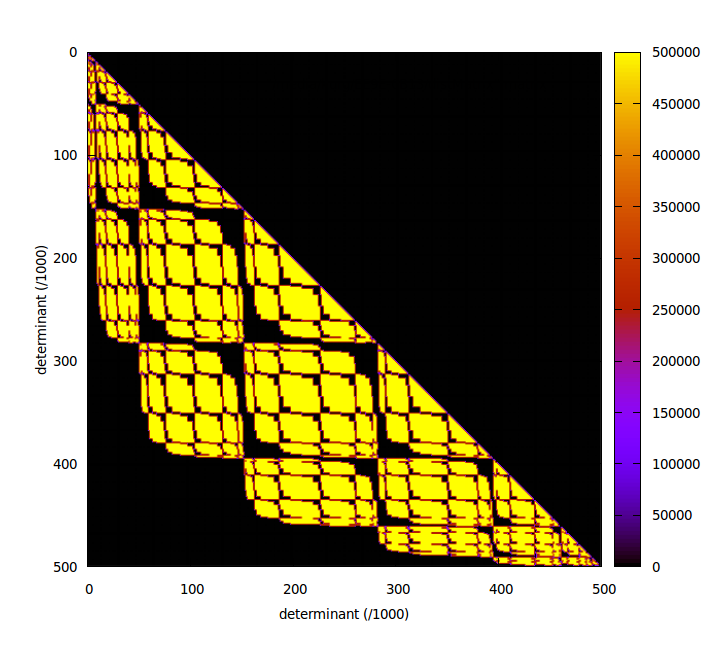
\includegraphics[width=0.6\columnwidth]{figures/davidson/num_subspace3}
		\caption{{\label{fig:num_subspace3}
		}}
	\end{center}
\end{figure}


\section{A few methods of interest}

A few methods happened to be of interest
\subsection{Highest electrons}
This method hasn't been explored throughoutly, but is still mentioned as it showed potentially interesting results, and can be use in combination with other methods.
The highest electrons are the most mobile ones, so they are the most likely not to match between two determinants. 

\begin{itemize}
	\item
$n \geq 3$ is a parameter of the method. 
	\item
$\mathcal{T}$ is a set of $n \geq 3$ electrons. 
	\item
$C(D)$ returns the set of the $n$ highest occupied spinorbitals of $D$. To make this unambiguous, it is arbitrarily decided that $\alpha$ spinorbitals are considered higher than their $\beta$ counterpart of same index.
	\item
$p(x, y) = n - |x \wedge y)| \leq 2$
\end{itemize}

$n$ is typically 3 or 4, as a larger value will result in lots of singletons, and the whole point of grouping determinants into sets being defeated. In the extreme case where $n = N_{electron}$, $C(D) = D$
   


\subsection{Singly occupied orbitals}
If there are $n$ orbitals that are singly occupied in $\ket I$ and not singly occupied in $\ket J$, it will take at least $n$ excitations to excite between $\ket I$ and $\ket J$.

\begin{itemize}
	\item
$\mathcal{T}$ is a set of orbitals
	\item
$C(D)$ returns the set of singly occupied orbitals in $D$
	\item
%$p(x, y) = max \big [popcnt(iand(x, z)), popcnt(iand(y, z)) \big ] > 2 ; z = ieor(x, y)$
$p(x, y) = max (|x|, |y|) - |x \wedge y| \leq 2$
\end{itemize}

Matrix $M$ for that method is shown in figure \ref{fig:xor_subspace}.
This method has one interesting property. If we compare determinants only with those contained in the same set - which is a tiny fraction of the total number of comparisons to be performed - we are guaranteed to find all excitations of the form $\hat T_{a \bar a}^{b \bar b}$ and $\hat T_{a \bar b}^{b \bar a}$, which are typically the largest non-diagonal matrix elements. Indeed, those excitations imply there was no change in singly occupied orbitals. And since they are the only one to do so, we are also guaranteed not to find any other type of excitation within a set.

\begin{figure}[H]
	\begin{center}
		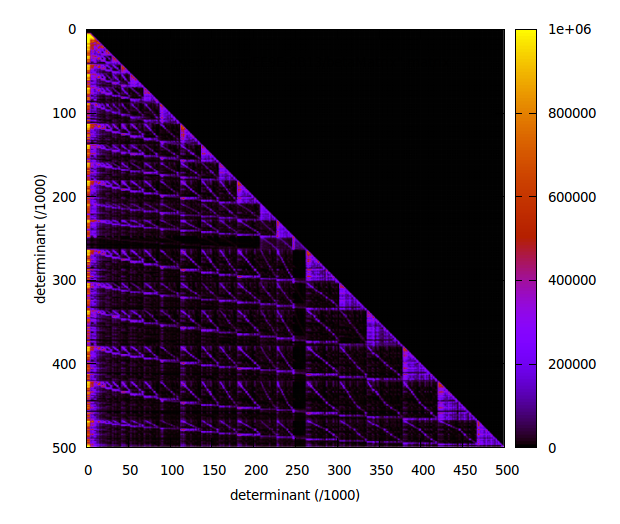
\includegraphics[width=0.6\columnwidth]{figures/davidson/xor_subspace}
		\caption{{\label{fig:xor_subspace}
		}}
	\end{center}
\end{figure}


\subsection{Simple spin part}
This methods has been implemented but was overriden by Composite spin part, introduced next. It is mostly mentioned for comprehension.

\begin{itemize}
	\item
$\mathcal{T}$ is a set of $\alpha$ spinorbitals
	\item
$C(D)$ returns $D_\alpha$, the set of occupied $\alpha$ spinorbitals in $D$
	\item
$p(x, y) = \frac{|x \oplus y|}{2} \leq 2$
\end{itemize}

$\frac{|x \oplus y|}{2}$ computes the excitation degree between $x$ and $y$ spin parts. 
    

    
\subsection{Composite spin part}
What can be noticed in the previous method, is that when we compute $p(x, y)$ to check if two sets $S_x$ and $S_y$ are disconnected, the value returned is the excitation degree for the $\alpha$ part between any $D_1 \in S_x$ and $D_2 \in S_y$. If $p(x, y)=2$, it means, $D_1$ and $D_2$ can only be connected if the excitation for the $\beta$ part is 0, in other words, if they share the same $\beta$ part. This in turn means that, when we compare determinants from $S_x$ and $S_y$, we are only looking for determinants with equal $\beta$ spin part.
Had we chosen $C(D)$ to return the $\beta$ spin part instead of the $\alpha$ one, $D_1$ and $D_2$ would have ended in the same set.
Taking this into account, we can set up a method that is made of two sub-methods, each one finding of a subset of possible excitations.

\begin{itemize}
\item
Find all connections between determinants that share the same $\alpha$ spin part. In other words, it finds all purely $\beta$ excitation,$\hat T_{\bar a}^{\bar b}$ and $\hat T_{\bar a \bar b}^{\bar c \bar d}$
\begin{itemize}
	\item
$\mathcal{T}_\alpha$ is a set of $\alpha$ spinorbitals
	\item
$C_\alpha(D)$ is the set of occupied $\alpha$ spinorbitals in $D$
	\item
%$p_\alpha(x, y) = max \big [popcnt(iand(x, z)), popcnt(iand(y, z)) \big ] > 2$, with $z = ieor(x, y)$
$p_\alpha(x, y) = (x = y)$
\end{itemize}
\item
Find all connections between determinants that are at most singly excited in their $\beta$ part.
This includes purely $\alpha$ excitation as well as $\alpha+\beta$ ones, $\hat T_a^b$, $\hat T_{ab}^{cd}$ and $\hat T_{\bar a b}^{\bar c d}$.
\begin{itemize}
	\item
$\mathcal{T}_\beta$ is a set of $\beta$ spinorbitals
	\item
$C_\beta(D)$ is the set of occupied $\beta$ spinorbitals in $D$
	\item
$p_\beta(x, y) = \frac{|x \oplus y|}{2} \leq 1$
\end{itemize}
\end{itemize}
    

All types of double excitations are found by either sub-method. The resulting $M$ matrices are shown in figures \ref{fig:aabb_subspace} and \ref{fig:ab_subspace}.
The point of this method compared to the previous one, is that the $p$ condition is drastically tightened, resulting in many more sets being by construction disconnected. For the simple spin part method, given a spin part $x$, the cardinality of the set of all $y$ spin parts so that $p(x, y) = TRUE$ is the number of possible double excitations. For composite spin part, it is respectively 1 ($p_\alpha$) and the number of single excitations ($p_\beta$).
As can be seen, the first method, although it finds all purely $\beta$ excitations, and could as well be used to find purely $\alpha$ ones, explores a minuscule area of $H$. As a matter of fact, finding those is pretty much "free", the vast majority of computational time is spent finding $\alpha \beta$ excitations.
As previously seen, the most important of excitations, those of the form $\hat T_{a \bar b}^{b \bar a}$, happen to be $\alpha \beta$ ones and can also be obtained for a very small cost using the singly occupied orbitals method. ( et donc? )

    
   
\begin{figure}[H]
	\begin{center}
		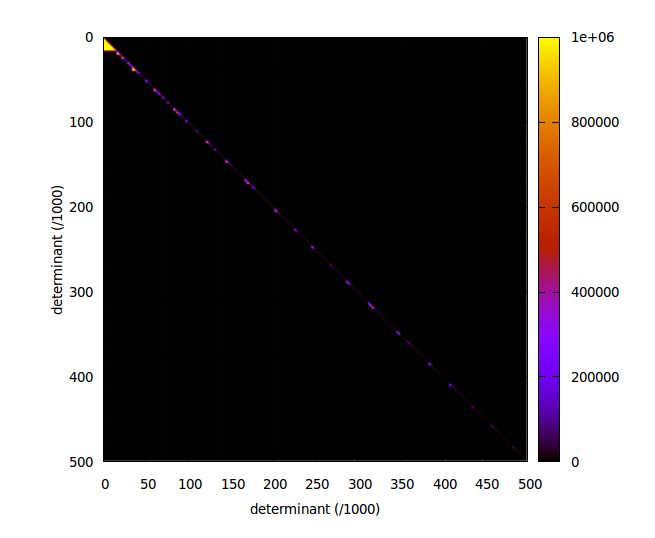
\includegraphics[width=0.6\columnwidth]{figures/davidson/aabb_subspace}
		\caption{{\label{fig:aabb_subspace}
		}}
	\end{center}
\end{figure}

\begin{figure}[H]
	\begin{center}
		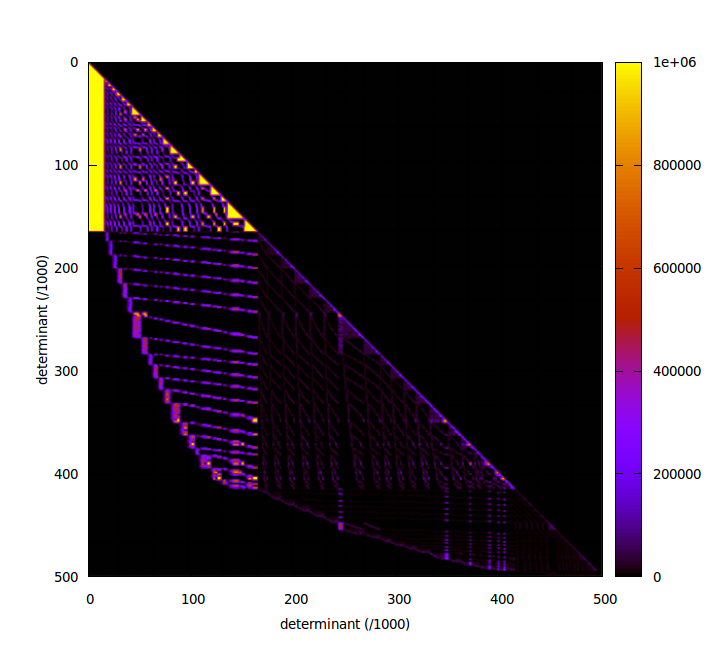
\includegraphics[width=0.55\columnwidth]{figures/davidson/ab_subspace}
		\caption{{\label{fig:ab_subspace}
		}}
	\end{center}
\end{figure}

\end{document}
